\chapter{Deep Learning}
Deep Learning describes a family of learning techniques
that at their core are about learning representations of data
in a hierarchical fashion.
It replaces the need for handcrafted feature
and indeed works in an entirely unsupervised or at least
semi-supervised fashion.
In this way,
it is often deployed as end-to-end learning
because it can learn its own higher-level abstractions
from raw data.

The core algorithm in deep learning is backpropagation
(described in detail in \ref{sec:backprop})
which describes how a learning model should update its parameters
in response to a discrepancy between learned output
and example output.

\paragraph{}
While the notion of stacking layers of units
to create multi-tiered artificial neural networks
has been around for a few decades already,
% TODO ref first Ann?
the recent surge in computing power
has enabled these conceptual models
to be actually built large enough
to explore their full potential.

Next to fully connected neural networks,
there are a few other types of networks of interest
that I will explore.
One such is the Convolutional Neural Network
which I will describe in more detail in
section \ref{sec:cnn}.
This type especially has benefitted from
advances in technology because of their highly
parallel nature which effectively allows them to be run
on consumer graphic hardware which is ever-improving
and becoming more accessible.

\paragraph{}
The areas that have benefited most from
this branch of machine learning
include without doubt
image recognition and speech recognition,
both problems with extremely noisy real-world data
that were typically tackled
by hand-crafting higher level features
and learning from those,
yet it is far from limited to these.
Deep learning has been extensively and successfully
applied to reinforcement learning as well,
the main topic of interest in this thesis.
In section \ref{sec:drl}
I will describe
the latest advances and current struggles
the deep reinforcement learning faces,
as well as my own attempts at improving
the current situation.


\section{Convolutional Neural Networks}
\label{sec:cnn}
The core to deep learning is that representations
of data can be learned in an unsupervised manner.
Convolutional networks are able to learn features
from raw input without any human intervention.
Stacking convolutional layers even allows
hierarchical features to be learned.
This way the initial layer could function
as an edge detector
whereas deeper layers
would learn higher-level abstractions
such as for example facial features
in the case of image recognition.

Another core property of convolutional layers is that,
unlike a regular fully connected neural network,
it can recognize the same features
regardless of the location of the feature in the input.
A regular fully connected network would need to have
its weights in each of the possible locations trained to recognize the same feature
which is wasteful in both space and computational requirements.

\paragraph{}
Convolutional networks are strongly inspired
by the animal visual cortex which contains two basic cell types.
Simple cells activate respond most strongly to edge patterns;
they function as edge-detectors and have a small receptive field.
Complex cells on the other hands have a larger receptive field
and are also spatially invariant to pattern location.

An early predecessor of the convolutional network
that tried to capture these concepts
is the neocognitron
\parencite{Fukushima1980}
which differs mostly in that convolutional networks
share weights across several positions in the input,
as I will explain further down.
The architecture I will explain in the following section
is based on the famous LeNet-5,
designed by
\citeauthor{LeCun1998}
(\citeyear{LeCun1998})
to successfully recognize hand-written letters.

\section{Building Blocks}
\label{sec:building_blocks}

\subsection{Convolutional Layer}
The core building block for a convolutional network
is the convolutional layer.
For the remainder of this text it is easiest
to think of input as images, possibly
with a depth dimension (such as color).

\begin{figure}[htpb]
  \centering
  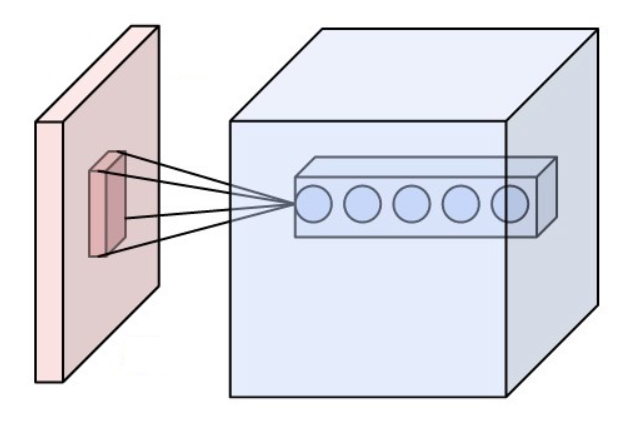
\includegraphics[width=0.7\linewidth]{conv_layer.png}
  \caption{Convolutional layer (blue) connected to an input layer.
    Highlighted are multiple filters connecting to a single input tile.
  }
  \label{fig:conv_layer}
\end{figure}

\paragraph{}
Let us start with the notion of a single, trainable neuron
in the convolutional layer.
It connects to only a small part of
the underlying input layer
as demonstrated in
Figure \ref{fig:conv_layer},
albeit through the whole depth.
This is the receptive field
as I described earlier.
Strongly connecting to only a small part of the input
is what allows convolutional networks
to exploit strong local correlations
that are inherently present
in natural images
but also in many other forms of
naturally occurring data.

\paragraph{}
This single neuron is part of a filter
that spans the whole input image,
it has neighbors that just like it
fully connect to neighboring patches of input.
One such a filter is now a flat 2D activation map
for a single feature.
This replication for a single filter
is what makes convolutional networks
insensitive to the location of a feature.

Of course we would like to have multiple features,
so we stack multiple of these filters on top of one another.
This stacking behavior of filters is described in
Figure \ref{fig:conv_layer},
where a single input patch is shown to correspond
to several filters.

\subsection{Parameter Sharing}
\label{sub:parameter_sharing}
As stated before, one feature corresponds to neurons across
the whole input by each corresponding to some patch of it.
This relies on the assumption that the feature could arise
anywhere in the input and would be useful to discover anywhere.
In order to actually compute the same feature,
we constrain the weights and bias of the neurons for a single feature
to be shared.

\subsection{Details}
\label{sub:details}
To actually generate the feature map
we \textit{convolve} the input with a linear filter,
add a bias and afterwards apply a non-linear function
such as a rectifier
(described in Section \ref{sec:relu}).
It is only because the weights are shared across a single feature
that this convolution is possible,
hence the name of the layer.

\paragraph{}
A single feature map $k$ in terms of its input $x$ could be computed as:

\begin{equation}
  h_k = tanh((W_k \cdot x) + b_k)
\end{equation}

It is also this operation that allows convolutional networks
to run so efficiently on parallel hardware,
making it the ideal candidate
for general purpose GPU computing.

\subsection{Tuning}
A single convolutional layer
has some hyperparameters that are both important
and hard to tweak.
Since learning a convolutional network
is still a rather slow endeavour,
it is best to start out with good estimates from the deep learning community.

\paragraph{}
The common way to build a convolutional network
from convolutional layers is to have
the layers closer to the input compute
few features,
computed over large receptive fields or tiles.
As the network grows deeper,
inputs to layers represent higher level features
and can thus be combined with less at a time;
intuitively, a few high-level features
can contain the same information of more
lower-level features.
Conversely, while there are only few
worthwhile raw features such as different types of edges,
there are probably more distinct higher-level features
that can be used to generate the final output.
Deeper layers should thus grow deeper yet slimmer spatially.

This setup typically results in a funnel-like structure
such as shown in Figure \ref{fig:conv_layer_funnel}.
The deepening occurs because of the increase in features
whereas the slimming usually occurs because multiple
outputs from an input layer correspond to only a single
neuron, spatially, in the next layer.
However, there are ways to train a neuron on a patch of input
yet still retain output size (again, spatially).
These I will describe below.

\begin{figure}[htpb]
  % TODO attribute to Hausknecht2015
  % TODO no seriously create new
  \centering
  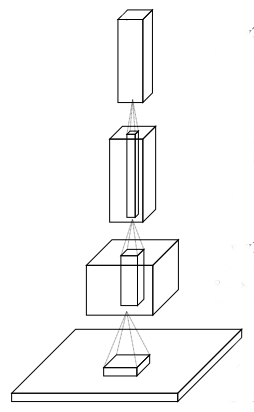
\includegraphics[width=0.3\linewidth]{conv_layer_funnel.png}
  \caption{Convolutional layers are often stacked
    in a funnel-like manner,
    growing smaller spatially
    yet larger in the depth or feature dimension.
  }
  \label{fig:conv_layer_funnel}
\end{figure}

\paragraph{}
As noted, both the amount of features
as well as the size of the receptive field in a layer
play a huge role in the representational capacity of the layer.
Still, there are other ways to affect this.
\begin{description}
  \item[Stride]
    The stride for a convolutional layer determines the spacing
    between receptive fields, or tiles.
    A stride of 1 would have very strongly overlapping tiles
    and as a result larger spatial dimensions
    than a lower stride would have.
    A stride equal to the tile size
    would result in non-overlapping but touching tiles.
    An even larger one would, of course,
    result in unused input elements and is therefore
    rather unpopular in practice.
  \item[Padding]
    If not all input elements can be used
    because of the filter size or the combination
    of filter size and stride,
    one can choose to pad the input with zeroes
    to achieve a valid convolution.
\end{description}

\subsection{Pooling Layer}
An important yet simpler concept to
convolutional networks is pooling,
a non-linear downsampling of the input.
The most popular form is max pooling,
demonstrated in Figure \ref{fig:maxpool}.

\begin{figure}[htpb]
  \centering
  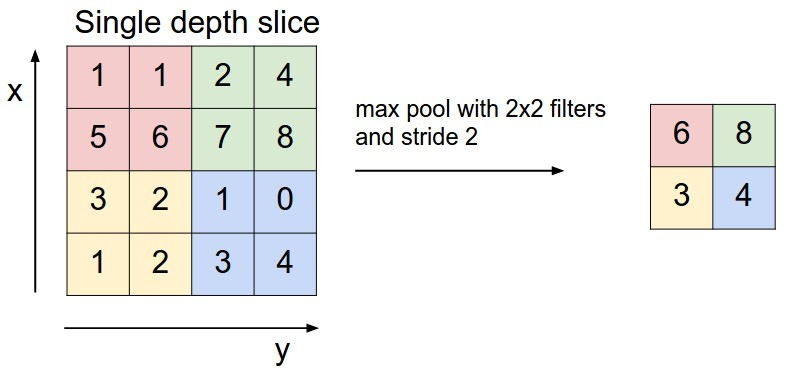
\includegraphics[width=0.7\linewidth]{maxpool.jpg}
  \caption{Max pooling with a filter size of $2 \times 2$
    and stride $2$.
  }
  \label{fig:maxpool}
\end{figure}

\paragraph{}
Pooling reduces the spatial size
while retaining the depth
as the depth describes the amount of features.
The idea behind the concept
is that spatial location of a feature is less important
than the activation of the feature
(note again the importance of translation invariance),
along with the notion that features are most important
in relation to other features.
Pooling therefore preserves relative location of each feature.

\paragraph{}
Even though most convolutional networks
tended to have pooling layers,
if not occasionally in between convolutional layers
then often right after them,
in recent years in the literature
there has been a tendency to avoid pooling layers altogether.
\citeauthor{Springenberg2015}
(\citeyear{Springenberg2015})
suggest that pooling does not always improve performance
if the network already has enough capacity for the data at hand
and indeed advocate the use of convolutional layers
with larger strides
and even more convolutional layer
to make up for the loss in power.

\section{Recurrent Neural Networks}

\section{Deep Reinforcement Learning}
\label{sec:deep_reinforcement_learning}



\section{Misc, still needs a decent place}
\subsection{RMSProp}
\label{sub:rmsprop}


